% Mangroves Thesis Poster
% Vincent Paul Fiestada & Andrew Vince Lorbis
% Copyright March 2017
% This document uses the SCL LaTeX Poster Class v1.1

\documentclass[a0paper,portrait]{scl-poster}
\usepackage[SCLcolors1]{SCLpostersetup}
\usepackage{graphicx}
\usepackage{float}

\begin{document}
\begin{poster}
%****************************************************************
%SETTINGS (Note: Please do not edit linebreaks and spaces within this section!)
%
%GENERAL POSTER SETTINGS
{%
  columns=3,
  headerheight=0.12\textheight, %top header, default = 0.1\textheight
  linewidth=1pt   %for posterbox 
}%
 
%TITLE HEADER SETTINGS
{\color{white}\bf\huge %xxxxxxxxxxxxxxx
%TITLE------------------------------------------
Agent-based Model Of Mangrove Forest Regrowth
%-----------------------------------------------
\\[0.005em]}   %xxxxxxxxxxxxxxxxxxxxxxxxx
{\color{white}{%xxxxxxxxxxxxxxxxxxxxxxxxx
%AUTHOR-----------------------------------------
Vincent Paul Fiestada$^1$, Andrew Vince Lorbis$^1$ and Vena Pearl A. Bongolan, Ph.D.$^1$
%----------------------------------------------------
}\\[0.2em]\small %xxxxxxxxxxxxxxxxxxxxxx
%INSTITUTE--------------------------------------
$^1$Scientific Computing Laboratory, Department of Computer Science, University of the Philippines Diliman\\
%-----------------------------------------------
\\\tt %xxxxxxxxxxxxxxxxxxxxxxxxxxxxxxxxx
%EMAIL-------------------------------------------
vffiestada@up.edu.ph, aalorbis@gmail.com, bongolan@dcs.upd.edu.ph
%-----------------------------------------------
}
%LOGO (the logo on the right)
{
\dcsscllogowhite
%\dcsscllogo
}
%****************************************************************



%POSTER BODY------------------------------------
\begin{posterbox}[name=intro,column=0,row=0]{Introduction}
Mangrove forests along tropical coastlines frequently suffer severe damage due to storms. The mangrove trees are extremely sensitive to environmental stressors such as water salinity and tidal inundation. We propose an agent-based model for the prediction of the regenerative behavior of mangrove stands consisting of the native species and the planted or non-native species in a fragmented habitat, with the use of spatio-temporal colored noise for stochastic seedling dispersal.
\begin{figure}[H]
  \centering
  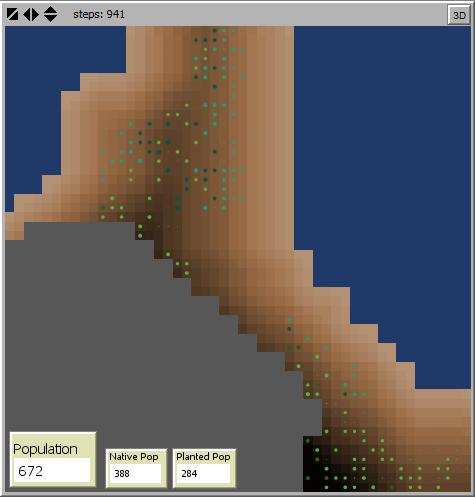
\includegraphics[width=0.85\textwidth]{graphics/screenshot1}
    \caption{Screenshot of the model during a run}
\end{figure}
\end{posterbox}

\begin{posterbox}[name=lists,column=0,below=intro]{Model Parameters}
The following are the global variables and agent parameters that affect the dynamic simulation of individual mangrove growth.\\
\begin{itemize}
  \item{Tree Variables \& Parameters}
    \begin{itemize}
      \item{Diameter $D$ (at breast height)}
      \item{Alpha $\alpha$ (relates Diameter to tree height)}
      \item{Beta $\beta$ (relates Diameter to crown radius)}
      \item{Gamma $\gamma$ (related to maximum height)}
    \end{itemize}
  \item{Species Parameters}
    \begin{itemize}
      \item{Omega $\Omega$ (conversion factor)}
      \item{$D_{max}$ or maximum attainable $D$}
      \item{Salinity sensitivity}
      \item{Inundation sensivity}
      \item{Competition sensitivity}
    \end{itemize}
  \item{Patch Variables}
    \begin{itemize}
      \item{Fertility (Boolean - This is \textit{true} if a plant can grow on the patch)}
      \item{Recruitment Chance}
      \item{Salinity}
      \item{Inundation}
    \end{itemize}
  \item{Global Variables}
    \begin{itemize}
      \item{$\delta t$ - Poission distributed time increment for each step of the simulation}
    \end{itemize}
\end{itemize}
\vspace{0.7em}
Plants also have a chance of dying during storms, which occur as Poission-distributed block disturbances throughout the simulation. Mature trees have a much greater chance of dying from storms than young plants. A tree's neighbors decreases its chances of dying during storms.
\end{posterbox}

\begin{posterbox}[name=overview,span=2,column=1,row=0]{How the Model Works}
The main state variable of the mangrove agents is their $D$. Growth is determined by the equation elaborated by Salmo and Juanico \cite{mangroveModelPaper}.
\begin{equation}
	\frac{dD}{dt} = \left(\frac{\Omega}{2 + \alpha}\right)D^{\beta - \alpha - 1} \left[1 - \frac{1}{\gamma}\left(\frac{D}{D_{max}}\right)^{1 + \alpha}\right] \times \sigma(x,y) \times \eta(x,y) \times K(x,y)
\end{equation}\\
Where $\sigma, \eta, K$ are the responses to salinity, inundation, and competition, respectively.
The simulation occurs in a 2D grid of patches, where each patch can be occupied by at most 1 plant (mangrove). Patches can represent coastal forest land, the sea, or human-claimed land. To start, mangroves are planted randomly on specified regions of coastal land. 
The time advances based on a Poisson random time increment with mean = 1 day, as per the model by \cite{mangroveModelPaper}. During each step, all mangroves grow according to the equation above and proportional to the random time increment.
Mangroves also die from natural causes with a mortality rate dependent on species and maturity as determined by the diameter. Storms can also cause the death of entire blocks of mangroves. In general, seedlings have a higher mortality rate while trees are more susceptible from storms, in particular isolated ones.
Each unoccupied livable patch has a chance of "recruiting" a new mangrove. Initially, this chance is zero, but it changes as a spatiotemporal stochastic variable, spreading out from patches with mature trees.
\end{posterbox}

\begin{posterbox}[name=significance,column=2,below=overview]{Significance}
Mangroves have great ecological significance. Deforestation threatens coastal forest ecosystems due to the key role that mangroves play as nurseries for fish and as keystone species of its ecosystem. Efforts to rehabilitate damaged mangrove forests involve important decisions, including the choice of species to plant. The model aims to provide insights into the regeneration behavior of non-native species introduced to a coastal area, which could be helpful in the decision-making process of conservationists.
\end{posterbox}

\begin{posterbox}[name=experiments,column=1,below=overview,above=bottom]{Experiments and Results}
We conducted several experiments, including sensitivity analysis with the model.
\end{posterbox}

\begin{posterbox}[name=refs,column=2,below=significance,above=bottom]{References}
% In the last box, you will usually have a list of references
% The bibliography automatically adds the title "References", but
% this have been removed in the preamble

% \vspace{0.7em}

% or uncomment below, if you are usin a .bib file:
{\scriptsize\singlespacing
\bibliographystyle{plain}
\bibliography{references}}
\end{posterbox}


\end{poster}
\end{document}
